\chapter{Hubo-Ach Manual}\label{sec:huboAchManual}
This section gives the prerequisites for the Hubo-Ach system, shows the user how to install/un-install the system, and how to use the built in tools.  Programming examples in C/C++ and Python are also given.

\section{Prerequisites}

The following items are needed to run Hubo-Ach on a Hubo:
\begin{itemize}
\item Hubo2+ or OpenHubo (Virtual Hubo)
\item SocketCAN compatible CAN card
\item Debian based linux install - tested with Ubuntu 12.04 LTS
\item Ach IPC installed
\end{itemize}




\section{Installation}
\subsection{From Hubo-Ach Dep (Recommended)}

\subsubsection{Updates to latest release:}
\begin{code}
$ hubo-ach update
\end{code}

\subsubsection{Updates to latest develop:}
\begin{code}
$ hubo-ach update develop
\end{code}

\subsubsection{From Repo:}
(1) Add one of the two lines to \textit{/etc/apt/sources.list}
\begin{code}
deb http://www.repo.danlofaro.com/release precise main \# Development
deb http://www.drc-hubo.com/release precise main \# Stable Release 
\end{code}

(2) Install via apt-get:
\begin{code}
$ sudo apt-get update
$ sudo apt-get install hubo-ach hubo-dev
\end{code}
or
\begin{code}
$ hubo-ach update apt-get
\end{code}

\subsection{From Source}
\subsubsection{Install from source}
Download the source and install
\begin{code}
$ git clone https://github.com/hubo/hubo-ach.git
$ cd hubo-ach
$ autoreconf -i
$ ./hubo-ach-install.sh
\end{code}

\subsubsection{Uninstall/Clean Hubo-Ach}
Removed all Hubo-Ach version from deb, apt-get and source
\begin{code}
$ hubo-ach clean
\end{code}











\section{Usage}

Starting Hubo-Ach will automatically start the interface between hubo and the user called hubo-console
\subsection{Hubo-Ach Main Interface}

\subsubsection{Available commands}
\begin{code}
$ hubo-ach
\end{code}

Start Hubo-Ach on Hubo
\begin{code}
$ hubo-ach start
\end{code}




\subsubsection{Start Hubo-Ach on OpenHubo (Virtual Hubo)}
\begin{code}
$ hubo-ach virtual
\end{code}



\subsection{Update Hubo-Ach}
\subsubsection{Updates to latest release:}
\begin{code}
$ hubo-ach update
\end{code}



\subsubsection{Updates to latest develop:}
\begin{code}
$ hubo-ach update develop
\end{code}

\subsubsection{Updates via apt-get}
Dependent on your apt-get entry in \textit{/etc/apt/source.list}:
\begin{code}
deb http://www.repo.danlofaro.com/release precise main # Develop
deb http://www.drc-hubo.com/release precise main # Stable
\end{code}

\begin{code}
$ hubo-ach update apt-get
\end{code}


\subsubsection{Remove Hubo-Ach}
Removed all installed versions of Hubo-Ach including from source.
\begin{code}
$ hubo-ach clean
\end{code}




\subsubsection{Start Hubo-Ach Console}
\begin{code}
$ hubo-ach console
\end{code}



\subsubsection{Start Hubo-Ach Read Tool}
\begin{code}
$ hubo-ach read
\end{code}


\subsubsection{Start Remote Connection}
Connection is made from the client to the server where the robot is the server. The robot's has an IP address of xxx.xxx.xxx.xxx and is the hubo-ach computer. Note: you have to have to enable the network daemon via the process described here: http://golems.github.com/ach/manual/\#AEN399
\begin{code}
$ hubo-ach remote xxx-xxx-xxx-xxx
\end{code}



Kill Remote Connection
\begin{code}
$ hubo-ach remote kill
\end{code}



\subsubsection{Make Ach Channes}
Creates Ach channels for Hubo-Ach without starting the Hubo-Ach Daemon
\begin{code}
$ hubo-ach make
\end{code}



\subsection{Hubo-Console}
Hubo-Console is a basic user interface between the Hubo and the user. It allows you to do the following:
\begin{itemize}
\item Home a single joint
\item Home all joints at once
\item Reset joint errors
\item Initialize sensors
\end{itemize}
Note: In all examples below XXX stands for the standard joint naming i.e. RHP, RHR, LSP, LSR, etc.
Hubo-Console will start automatically when you type:
\begin{code}
$ hubo-ach start
\end{code}


If Hubo-Ach is already started you can start hubo-console by:
\begin{code}
$ hubo-ach console
\end{code}




Once Hubo-Console has started you will be able to:


\subsubsection{Home Joint XXX}
This will make the joint move to find the limit switch then goto its predefined offset. The reference will be set to zero.
\begin{code}
>> hubo-ach: home XXX
\end{code}




\subsubsection{Home All Joints}
This will make all of the joints move to find their respective limit switches and goto their predefined offsets at the same. The reference to all joints are set to zero. Note: All joints will move at the same time. The rotbot should not be on the ground when this is done.
\begin{code}
>> hubo-ach: homeAll
\end{code}



\subsubsection{Initialize All Sensors}
This will initialize all sensors including the IMU and FT sensors. The robot should be off the ground and not moving.

\begin{code}
>> hubo-ach: iniSensors
\end{code}



\subsubsection{Initialize All joints}
This will initialize all joints. Note: They will maintain the current control mode. If they were inactive they will be active and able to read back encoder values at this point.
\begin{code}
>> hubo-ach: initializeAll
\end{code}

\subsubsection{Clear Errors on Joint XXX}
This will clear the following errors on joint XXX.
\begin{itemize}
\item Big Error
\item Encoder Error
\item Homing Error
\end{itemize}

\begin{code}
>> hubo-ach: reset XXX
\end{code}



\subsubsection{Clear Errors on All Joints}
This is the same as reset but will clear errors on all active joints
\begin{code}
>> hubo-ach: resetAll
\end{code}



\subsubsection{Joint XXX goto position}
Commands joint XXX to goto position YYY (in radians)
\begin{code}
>> hubo-ach: goto XXX YYY
\end{code}

\subsubsection{Turn on/off Joint XXX Controller}
This will turn on or off the controller for joint XXX.
Note: Y represents the desired state
\begin{itemize}
\item 1 = on
\item 0 = off
\end{itemize}

\begin{code}
>> hubo-ach: ctrl XXX Y
\end{code}






\subsubsection{Turn on/off All Joint Controllers}
This is the same as Turn on/off Joint XXX Controller but it applies to all joints:

\begin{code}
>> hubo-ach: ctrlAll Y
\end{code}




\subsubsection{Check Status of Joint XXX}
Check the status of joint XXX
\begin{code}
>> hubo-ach: status XXX
\end{code}


\subsection{Hubo-Read}
Hubo-Read is a simple tool that prints out the reference and state channels to the console.
You can start Hubo-Read in one of two ways:
\subsubsection{Method 1}
\begin{code}
$ hubo-ach read
\end{code}

\subsubsection{Method 2}
Note: the sudo is needed because it uses RT permissions for the loop.

\begin{code}
$ sudo hubo-read
\end{code}

What you will see

\scriptsize
\begin{code}
t = 1363724430.086347873
WST : Cmd = 0.000000      Ref = 0.000000     Enc = 0.000000     Cur = 0.000000     Tmp = 0.000000    
NKY : Cmd = 0.000000      Ref = 0.000000     Enc = 0.000000     Cur = 0.000000     Tmp = 0.000000    
NK1 : Cmd = 0.000000      Ref = 0.000000     Enc = 0.000000     Cur = 0.000000     Tmp = 0.000000    
NKP : Cmd = 0.000000      Ref = 0.000000     Enc = 0.000000     Cur = 0.000000     Tmp = 0.000000    
LSP : Cmd = 0.000000      Ref = 0.000000     Enc = 0.000000     Cur = 0.000000     Tmp = 0.000000    
LSR : Cmd = 0.000000      Ref = 0.000000     Enc = 0.000000     Cur = 0.000000     Tmp = 0.000000    
LSY : Cmd = 0.000000      Ref = 0.000000     Enc = 0.000000     Cur = 0.000000     Tmp = 0.000000    
LEB : Cmd = 0.000000      Ref = 0.000000     Enc = 0.000000     Cur = 0.000000     Tmp = 0.000000    
LWY : Cmd = 0.000000      Ref = 0.000000     Enc = 0.000000     Cur = 0.000000     Tmp = 0.000000    
LWR : Cmd = 0.000000      Ref = 0.000000     Enc = 0.000000     Cur = 0.000000     Tmp = 0.000000    
LWP : Cmd = 0.000000      Ref = 0.000000     Enc = 0.000000     Cur = 0.000000     Tmp = 0.000000    
RSP : Cmd = 0.000000      Ref = 0.000000     Enc = 0.000000     Cur = 0.000000     Tmp = 0.000000    
RSR : Cmd = 0.000000      Ref = 0.000000     Enc = 0.000000     Cur = 0.000000     Tmp = 0.000000    
RSY : Cmd = 0.000000      Ref = 0.000000     Enc = 0.000000     Cur = 0.000000     Tmp = 0.000000    
REB : Cmd = 0.000000      Ref = 0.000000     Enc = 0.000000     Cur = 0.000000     Tmp = 0.000000    
RWY : Cmd = 0.000000      Ref = 0.000000     Enc = 0.000000     Cur = 0.000000     Tmp = 0.000000    
RWR : Cmd = 0.000000      Ref = 0.000000     Enc = 0.000000     Cur = 0.000000     Tmp = 0.000000    
RWP : Cmd = 0.000000      Ref = 0.000000     Enc = 0.000000     Cur = 0.000000     Tmp = 0.000000    
LHY : Cmd = 0.000000      Ref = 0.000000     Enc = 0.000000     Cur = 0.000000     Tmp = 0.000000    
LHR : Cmd = 0.000000      Ref = 0.000000     Enc = 0.000000     Cur = 0.000000     Tmp = 0.000000    
LHP : Cmd = 0.000000      Ref = 0.000000     Enc = 0.000000     Cur = 0.000000     Tmp = 0.000000    
LKN : Cmd = 0.000000      Ref = 0.000000     Enc = 0.000000     Cur = 0.000000     Tmp = 0.000000    
LAP : Cmd = 0.000000      Ref = 0.000000     Enc = 0.000000     Cur = 0.000000     Tmp = 0.000000    
LAR : Cmd = 0.000000      Ref = 0.000000     Enc = 0.000000     Cur = 0.000000     Tmp = 0.000000    
RHY : Cmd = 0.000000      Ref = 0.000000     Enc = 0.000000     Cur = 0.000000     Tmp = 0.000000    
RHR : Cmd = 0.000000      Ref = 0.000000     Enc = 0.000000     Cur = 0.000000     Tmp = 0.000000    
RHP : Cmd = 0.000000      Ref = 0.000000     Enc = 0.000000     Cur = 0.000000     Tmp = 0.000000    
RKN : Cmd = 0.000000      Ref = 0.000000     Enc = 0.000000     Cur = 0.000000     Tmp = 0.000000    
RAP : Cmd = 0.000000      Ref = 0.000000     Enc = 0.000000     Cur = 0.000000     Tmp = 0.000000    
RAR : Cmd = 0.000000      Ref = 0.000000     Enc = 0.000000     Cur = 0.000000     Tmp = 0.000000    
RF1 : Cmd = 0.000000      Ref = 0.000000     Enc = 0.000000     Cur = 0.000000     Tmp = 0.000000    
RF2 : Cmd = 0.000000      Ref = 0.000000     Enc = 0.000000     Cur = 0.000000     Tmp = 0.000000    
RF3 : Cmd = 0.000000      Ref = 0.000000     Enc = 0.000000     Cur = 0.000000     Tmp = 0.000000    
RF4 : Cmd = 0.000000      Ref = 0.000000     Enc = 0.000000     Cur = 0.000000     Tmp = 0.000000    
RF5 : Cmd = 0.000000      Ref = 0.000000     Enc = 0.000000     Cur = 0.000000     Tmp = 0.000000    
LF1 : Cmd = 0.000000      Ref = 0.000000     Enc = 0.000000     Cur = 0.000000     Tmp = 0.000000    
LF2 : Cmd = 0.000000      Ref = 0.000000     Enc = 0.000000     Cur = 0.000000     Tmp = 0.000000    
LF3 : Cmd = 0.000000      Ref = 0.000000     Enc = 0.000000     Cur = 0.000000     Tmp = 0.000000    
LF4 : Cmd = 0.000000      Ref = 0.000000     Enc = 0.000000     Cur = 0.000000     Tmp = 0.000000    
LF5 : Cmd = 0.000000      Ref = 0.000000     Enc = 0.000000     Cur = 0.000000     Tmp = 0.000000    
    : Mx = 0.000000     My = 0.000000     Fz = 0.000000    
    : Mx = 0.000000     My = 0.000000     Fz = 0.000000    
    : Mx = 0.000000     My = 0.000000     Fz = 0.000000    
    : Mx = 0.000000     My = 0.000000     Fz = 0.000000    
    : Ax = 0.000000     Ay = 0.000000     Az = 0.000000    
    : Ax = 0.000000     Ay = 0.000000     Az = 0.000000    
    : Ax = 0.000000     Ay = 0.000000     Wx = 0.000000     Wy = 0.000000
\end{code}
\normalsize























\section{Simulator}

This section shows how to run a Hubo simulator in conjunction with Hubo-Ach. Note: The simulator is a full 3D simulator and is recomended to run on a computer other the Hubo body computer. It will work on it but it will be slow.
\subsection{Prerequisites}

\subsubsection{OpenHubo}
To install OpenHubo follow the directions here: 
\begin{itemize}
\item http://dasl.mem.drexel.edu/drcwiki/index.php/OpenHubo\_Introduction
\end{itemize}

Assuming you have all of the prerequisites you can simply do the following to install OpenHubo:
\begin{code}
$ git clone --recursive https://github.com/hubo/openHubo.git
$ cd openHubbo
$ ./setup
\end{code}

\subsection{Using the Simulator}
Once OpenHubo is installed you can run run the simulator. The simulator at the moment is restricted to kinimatic output. Dynamics do not run in real-time. This simulator creates two models overlaid on each-other. The green model is the commanded reference sent to the actuator. The solid model is the actual position as read from the encoders. Note: if the robot is not on this will stay zero but the green reference will move.
To run the simulator:

\subsubsection{With No Physics (fast):}
Starts OpenHubo running with no physics. This is good for watching what the robot is doing live or to preview trajectories.
\begin{code}
$ hubo-ach sim openhubo nophysics
\end{code}

\subsubsection{With Physics:}
Starts OpenHubo running with physics. This runs at about 35\% real time (on an i7 processor). The simulator and hubo-ach are synced via triggering from newly received messaged on the following Ach channels:

\begin{itemize}
\item HUBO\_CHAN\_VIRTUAL\_TO\_SIM\_NAME
\item HUBO\_CHAN\_VIRTUAL\_FROM\_SIM\_NAME 
\end{itemize} 

Please note that the state channel will have simulation time NOT real time.

\begin{code}
$ hubo-ach sim openhubo physics
\end{code}

\subsection{Run Visualizer}
You can use OpenHubo as a real-time (live) visualizer of our state data on your computer in which you login to the Hubo from. This will show the OpenHubo model using no physics. The green shows what the joints are commanded to and the grey show where the joints are. This will run with little to no lag/latency on an i5 or i7 processor.
In order to do this start hubo-ach normally on the hubo:

\begin{code}
(hubo@xxx.xxx.xxx.xxx) $ hubo-ach start
\end{code}

On your control computer (not the hubo) start the simulator with remote
\begin{code}
(i5 or i7) $ hubo-ach sim openhubo nophysics remote xxx.xxx.xxx.xxx
\end{code}

















\section{Programming}

This section will show quick examples of how to program using Hubo-Ach in C/C++ and Python
\subsection{C/C++}\label{sec:ccppExample}
The C/C++ Example is available below. This is bare bones for you to:

\begin{itemize}
\item Get the latest feed-back (state) channel information.
\item Set the feed-forward (reference) information.
\end{itemize}


\footnotesize
\noindent \textbf{C/C++ Example (hubo-simple-demo.c)}
\vspace{-6mm}
\begin{code}
/* Standard Stuff */
#include <string.h>
#include <stdio.h>

/* Required Hubo Headers */
#include <hubo.h>

/* For Ach IPC */
#include <errno.h>
#include <fcntl.h>
#include <assert.h>
#include <unistd.h>
#include <pthread.h>
#include <ctype.h>
#include <stdbool.h>
#include <math.h>
#include <inttypes.h>
#include "ach.h"


/* Ach Channel IDs */
ach_channel_t chan_hubo_ref;      // Feed-Forward (Reference)
ach_channel_t chan_hubo_state;    // Feed-Back (State)

int main(int argc, char **argv) {

    /* Open Ach Channel */
    int r = ach_open(&chan_hubo_ref, HUBO_CHAN_REF_NAME , NULL);
    assert( ACH_OK == r );

    r = ach_open(&chan_hubo_state, HUBO_CHAN_STATE_NAME , NULL);
    assert( ACH_OK == r );



    /* Create initial structures to read and write from */
    struct hubo_ref H_ref;
    struct hubo_state H_state;
    memset( &H_ref,   0, sizeof(H_ref));
    memset( &H_state, 0, sizeof(H_state));

    /* for size check */
    size_t fs;

    /* Get the current feed-forward (state) */
    r=ach_get(&chan_hubo_state, &H_state, sizeof(H_state), &fs, NULL, ACH_O_LAST);
    if(ACH_OK != r) {
        assert( sizeof(H_state) == fs );
    }

    /* Set Left Elbow Bend (LEB) and Right Shoulder Pitch (RSP) */
    /* to  -0.2 rad and 0.1 rad respectively */
    H_ref.ref[LEB] = -0.2;
    H_ref.ref[RSP] = 0.1;

    /* Print out the actual position of the LEB */
    double posLEB = H_state.joint[LEB].pos;
    printf("Joint = %f\r\n",posLEB);

    /* Print out the Left foot torque in X */
    double mxLeftFT = H_state.ft[HUBO_FT_L_FOOT].m_x;
    printf("Mx = %f\r\n", mxLeftFT);

    /* Write to the feed-forward channel */
    ach_put( &chan_hubo_ref, &H_ref, sizeof(H_ref));

}

\end{code}
\normalsize


Where the default \textbf{MakeFile} is:

\footnotesize
\noindent \textbf{C/C++ Default MakeFile}
\vspace{-6mm}
\begin{code}
default: all

CFLAGS := -I./include -g --std=gnu99
CC := gcc

BINARIES := hubo-simple-demo
all : $(BINARIES)

LIBS := -lach 

hubo-simple-demo: src/hubo-simple-demo.o
	gcc -o $@ $< $(LIBS)

%.o: %.c
	$(CC) $(CFLAGS) -o $@ -c $<

clean:
	rm -f $(BINARIES) src/*.o
\end{code}
\normalsize

\subsubsection{Run the example}
The C/C++ example uses the MakeFile seen in Section~\ref{sec:ccppExample}. You just need to make and run

\begin{code}
$ make clean
$ make 
$ ./hubo-simple-demo
\end{code}










\subsection{Python}
The Python Example is available below. This is bare bones for you to:
\begin{itemize}
\item Get the latest feed-back (state) channel information
\item Set the feed-forward (reference) information
\end{itemize}

Please note that:
\begin{itemize}
\item Must use Hubo-Ach >= 0.0.20130319 
\item The Ach python bindings must be installed. You can install via PIP (see below)
\end{itemize}

\begin{code}
$ sudo apt-get install python-pip
$ sudo pip install http://code.golems.org/src/ach/py_ach-latest.tar.gz
\end{code}



\footnotesize
\noindent \textbf{Python Example (hubo-simple-demo.py)}
\vspace{-6mm}
\begin{code}
#!/usr/bin/env python
# /* -*-  indent-tabs-mode:t; tab-width: 8; c-basic-offset: 8  -*- */

import hubo_ach as ha
import ach
import sys
import time
from ctypes import *

# Open Hubo-Ach feed-forward and feed-back (reference and state) channels
s = ach.Channel(ha.HUBO_CHAN_STATE_NAME)
r = ach.Channel(ha.HUBO_CHAN_REF_NAME)
s.flush()
r.flush()

# feed-forward will now be refered to as "state"
state = ha.HUBO_STATE()

# feed-back will now be refered to as "ref"
ref = ha.HUBO_REF()

# Get the current feed-forward (state) 
[statuss, framesizes] = s.get(state, wait=False, last=False)

# Set Left Elbow Bend (LEB) and Right Shoulder Pitch (RSP) 
# to  -0.2 rad and 0.1 rad respectively
ref.ref[ha.LEB] = -0.2
ref.ref[ha.RSP] = 0.1

# Print out the actual position of the LEB
print "Joint = ", state.joint[ha.LEB].pos

# Print out the Left foot torque in X
print "Mx = ", state.ft[ha.HUBO_FT_L_FOOT].m_x

# Write to the feed-forward channel
r.put(ref)

# Close the connection to the channels
r.close()
s.close()
\end{code}
\normalsize

\subsubsection{Run the example}
The python example can be run via:

\begin{code}
$ python ./hubo-simple-demo.py
\end{code}




\section{Connecting a Simulator to Hubo-Ach}
This is a brief example of how to connect a simulator to Hubo-Ach. In this example we will be running Hubo-Ach in simtime mode. This makes Hubo-Ach wait for a trigger from the simulator. This trigger tells Hubo-Ach that it has updated the state data with the simulated state data. Hubo-Ach will then run and send a trigger to the simulator telling it that it can do its next calculation.

Hubo-Ach is simulator agnostic. The examples is given in this section uses the OpenHubo simulator described in Section~\ref{sec:simulator}

\subsection{Simulator}\label{sec:simulator}
	The simulator used for Hubo-Ach is the OpenHubo.
OpenHubo is an open-source kinematic and dynamic simulator for the the Hubo2 and Hubo2+ series robots.
It was developed by the Drexel Autonomous Systems Lab and runs using the open-source robot simulation environment OpenRAVE\cite{diankovThesis}.
Fig.~\ref{fig:openhubbo} shows the OpenHubo shell model and collision model.

\begin{figure}[thpb]
  \centering
      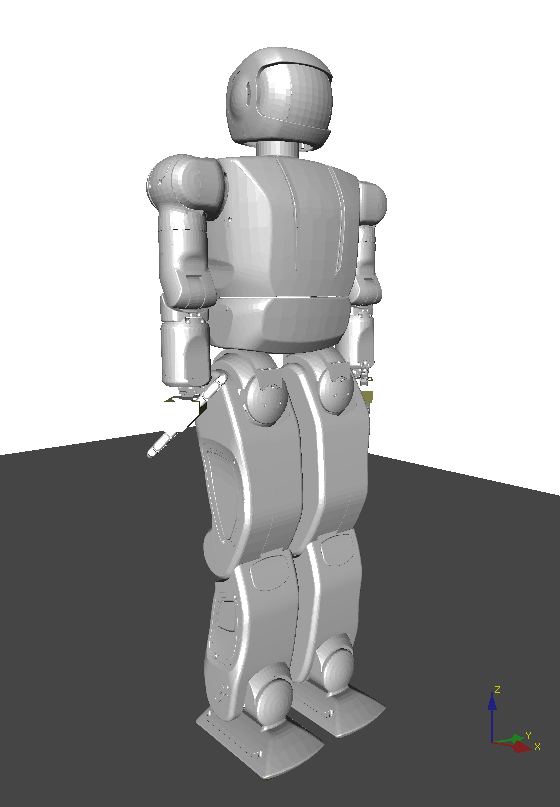
\includegraphics[width=0.4\columnwidth]{./pix/hBody.png}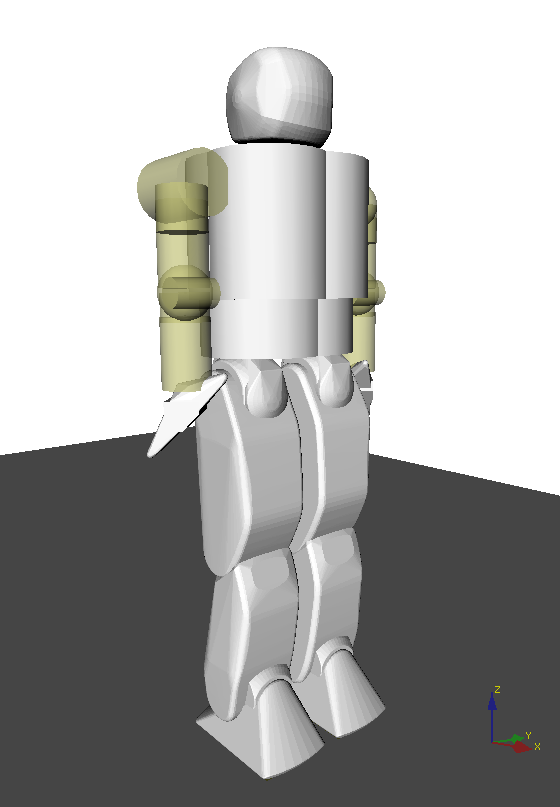
\includegraphics[width=0.4\columnwidth]{./pix/hCol.png}
      
\caption{OpenHubo model of the Hubo2 humanoid robot developed by the Drexel Autonomous Systems Lab and runs using the open-source robot simulation environment OpenRAVE\cite{diankovThesis}.  (Left) Shell Model - High polygon count.  (Right) Collision model - Made with primitives.}
\label{fig:openhubbo}
\end{figure}

The masses and lengths are of the OpenHubo model are all based off of the CAD model.
The shell model includes an external skin based off of the CAD model of the Hubo's shell.
This model is high polygon count and thus tends to require more processing time to detect collisions.
The collision model is constructed out of primitives in order to decrease the complexity of the model and decrease required processing time.
The collision model is a representation of the shell model. 
It does not precisely fit the contours but through experimentation and use has been calibrated to be a good representation of the Hubo's outer shell.

Fig~\ref{fig:openhubosim} shows the diagram of how the OpenHubo simulator is connected to Hubo-Ach.  
No changes to previous controllers are required for them to work with the simulator.
Just as before the desired reference $\theta_d$ being filtered before applied to Hubo via Hubo-Ach.  
$\theta_d$ is sent through a filter that reduces the \textit{jerk} on the actuator then the new reference $\theta_r$ is set on the \textbf{FeedForward} channel, Hubo-Ach reads it then commands Hubo at the rising edge of the next cycle.  
At this point the \textit{to simulator} trigger, $\Gamma_{ts}$, is set high and the OpenHubo simulator reads $\theta_c$.
The simulator waits until Hubo-Ach is ready until it starts its next set of cycles.
The reference is set within OpenHubo and solved with a simulation period of $T_{sim}$.
The simulation period $T_{sim}$ must be an integer deviser of the robot real-time period $T_r$.
In this case

\begin{equation}
T_r=0.005~s
\end{equation}

\begin{equation}
T_{sim} = \frac{T_r}{n}
\end{equation}


Once the simulator has gone through $n$ cycles the current state, $H_{state}$ is placed on the Hubo-Ach \textbf{FeedForward} channel and the ready trigger $\Gamma_{fs}$ is raised.  
Hubo-Ach is waiting for the rising edge of the \textit{from simulator} trigger, $\Gamma_{fs}$, to continue on to the next cycle.

\begin{figure}
\centering

\begin{tikzpicture}[->,>=stealth',shorten >=1pt,auto,node distance=5cm,
  thick,main node/.style={fill=white!20,draw,font=\sffamily\Large\bfseries}]


  \node[main node] (ctrl) {Controller};
  \node[main node] (filter) [right=1.5cm of ctrl] {Filter};
  \node[main node] (hubo-ach) [below=1.0cm of filter] {Hubo-Ach};
  
  \node[main node,font=\small] (hold1) [right=1.5cm of hubo-ach, yshift=0.5cm] {hold};
  \node[main node,font=\small] (hold2) [right=1.5cm of hubo-ach, yshift=-0.5cm] {hold};

  \node[main node] (hubo) [right=1.5cm of hold1, yshift=-0.5cm] {OpenHubo};




%  \path[->, every node/.style={font=\sffamily\small}]
%    (hubo-ach) edge node [above] {$\theta_c$} (hubo);

\draw[->] ([yshift=0.2 cm]hubo-ach.east)  to [out=0,in=-180] node [below] {$\theta_c$} ([yshift=-0.0 cm]hold1.west)  ;
\draw[->] ([yshift=0.0 cm]hold1.east)  to [out=0,in=-180] node [below] {$\theta_c$} ([yshift=0.2 cm]hubo.west)  ;
\draw[-*] ([xshift=1.0 cm]hubo-ach.north)  to [out=60,in=120] node [above] {$\Gamma_{ts}$} ([yshift=-0.05 cm]hold1.north)  ;



\draw[->] ([yshift=0.0 cm]hold2.west)  to [out=180,in=0] node [below] {$H_{state}$} ([yshift=-0.2 cm]hubo-ach.east)  ;
\draw[->] ([yshift=-0.2 cm]hubo.west)  to [out=180,in=0] node [below right] {$H_{state}$} ([yshift=0.0 cm]hold2.east)  ;
\draw[-*] ([xshift=0.0 cm]hubo.south)  to [out=-120,in=-60] node [above] {$\Gamma_{fs}$} ([yshift=0.05 cm]hold2.south)  ;

\draw[->] ([yshift=-0.0 cm]hubo-ach.west)  to [out=180,in=-90] node [below left] {$H_{state}$} ([yshift=0.0 cm]ctrl.south)  ;



%\draw[->] ([yshift=-0.2 cm]hubo.west)  -- node [below] {$H_{state}$} ([yshift=-0.2 cm]hubo-ach.east)  ;
%\draw[->] ([yshift=-0.0 cm]hubo.south)  to [out=-120,in=-60] node [below] {$\Gamma_{fs}$} ([yshift=-0.0 cm]hubo-ach.south)  ;



  \path[->,every node/.style={font=\sffamily\small}]
    (ctrl) edge node [above] {$\theta_d$} (filter);

 \draw[->] ([xshift=-0.5 cm]filter.south)  -- node [left] {$\theta_r$} ([xshift=-0.5 cm]hubo-ach.north)  ;
 \draw[->] ([xshift=0.5 cm]hubo-ach.north) -- node [left] {$\theta_a$} ([xshift=0.5 cm]filter.south)  ;


\end{tikzpicture}
\caption{Desired reference $\theta_d$ being filtered before applied to Hubo via Hubo-Ach.  $\theta_d$ is sent through a filter that reduces the \textit{jerk} on the actuator then the new reference $\theta_r$ is set on the \textbf{FeedForward} channel, Hubo-Ach reads it then commands Hubo at the rising edge of the next cycle.}
\label{fig:hubo-ach-feedforwardFilter}
\end{figure}




The external controllers do not know weather Hubo-Ach is running in \textit{simulation} or \textit{real-time} mode.  
In order to ensure a Hubo-Ach controller stays what ever timing method is being used the controller can do any of the following:

\begin{itemize}
\item Wait for the $\Gamma_{fs}$ trigger
\item Wait for a new $H_P{state}$ to be updated
\item Watch the time listed within $H_{state}$
\end{itemize}

If the given task does not require physics or feedback from $H_{state}$ then you can run in \textit{no physics} mode.
\textit{No physics} mode only gives collisions, joint angles and ideal feedback from the sensors.
In addition \textit{no physics} is capable of running much faster then real-time if needed.



\begin{table}
\centering
\caption{OpenHubo simulator sim-time and real-time comparison chart.  Shows the maximum percent real-time the OpenHubo simulator is capable of preforming at where 100\% is real-time.  All tests were preformed on an Intel i7 running at 2.8Ghz with 18Gb of RAM.}
\begin{tabular}{| l || c | c |}
\hline
Mode               & Timing                & Maximum Percent Real-Time (\%) \\
\hline
\hline
Physics            & Sim-Time              & 37\%   \\
\hline
No Physics         & Real-Time or Sim-Time & 362\%  \\
\hline
\end{tabular}\label{table:simtime}
\end{table}


Fig.~\ref{fig:huboOpenHuboWalking} shows the capability of Hubo-Ach to run in both sim-time and real-time modes.  
This is the same statically stable trajectory as seen in Section~\ref{sec:WalkingPatternGeneration}


\begin{figure}[thpb]
  \centering
      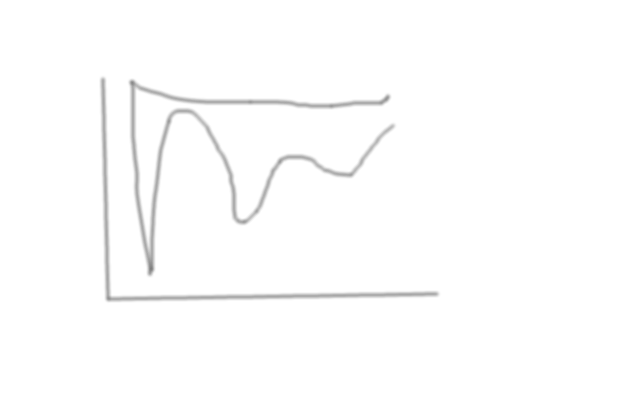
\includegraphics[width=0.69\columnwidth]{./pix/tmp.png}
      
\includegraphics[width=0.3\columnwidth]{./qrcode/qrcode-hubo-openhubo-walking.png}\\
      Video: http://danlofaro.com/phd/walking/\#WalkingHuboAndOpenHubo
\caption{Hubo and OpenHubo walking using Hubo-Ach in Real-Time and Sim-Time Respectively}
\label{fig:huboOpenHuboWalking}
\end{figure}


	
	

\subsection{Setup}

\subsubsection{Step 1: Start Hubo-Ach in SimTime mode}

This mode makes hubo-ach wait for a trigger from the simulator. This trigger is when the HUBO\_CHAN\_VIRTUAL\_FROM\_SIM\_NAME channel has been updated.
\begin{code}
$ hubo-ach sim
\end{code}


\subsubsection{Step 2: Run your simulator}

Run your simulator. The simulator must do the following in this order


\footnotesize
\noindent \textbf{(Sudo Code)}
\vspace{-6mm}
\begin{code}
Open all needed Channels
Write to HUBO_CHAN_VIRTUAL_FROM_SIM_NAME channel
Loop:
    Wait for HUBO_CHAN_VIRTUAL_TO_SIM_NAME channel update
    Set feed forward data from H_state.joint[jnt].ref to your simulator
    Do simulation
    Populate state data to H_state struct
        H_state.joint[jnt].pos
        H_state.imu[i].*
        H_state.ft[i].*
    Write H_state to HUBO_CHAN_STATE_NAME
    Write to HUBO_CHAN_VIRTUAL_FROM_SIM_NAME channel
    Goto Loop
\end{code}
\normalsize




\subsubsection{Step 3: Run a Hubo-Ach controller of your choosing}

You can now run any hubo-ach controller with no modification required. Note: If you want to take into account the simtime then it must either:
\begin{itemize}
	\item Watch the state time H\_state.time
	\item Wait for the following triggers:
	\begin{itemize}
		\item HUBO\_CHAN\_VIRTUAL\_FROM\_SIM\_NAME
		\item HUBO\_CHAN\_VIRTUAL\_TO\_SIM\_NAME
	\end{itemize}
\end{itemize}



\subsection{C/C++ Simulation Example}

This example code shows the basics of connecting to Hubo-Ach using simtime mode with triggering. The example can be found on the hubo group on github in the example/simtime branch:

\begin{code}
$ git clone https://github.com/hubo/hubo-simple-demo.git
$ cd hubo-simple-demo
$ git checkout example/simtime
\end{code}





\footnotesize
\noindent \textbf{C/C++ Simulation Example (hubo-simple-demo.c) - simtime branch}
\vspace{-6mm}
\begin{code}
/* Standard Stuff */
#include <string.h>
#include <stdio.h>

/* Required Hubo Headers */
#include <hubo.h>

/* For Ach IPC */
#include <errno.h>
#include <fcntl.h>
#include <assert.h>
#include <unistd.h>
#include <pthread.h>
#include <ctype.h>
#include <stdbool.h>
#include <math.h>
#include <inttypes.h>
#include "ach.h"

/* Ach Channel IDs */
ach_channel_t chan_hubo_ref;      // Feed-Forward (Reference)
ach_channel_t chan_hubo_state;    // Feed-Back (State)
ach_channel_t chan_hubo_to_sim;    // To Sim
ach_channel_t chan_hubo_from_sim;    // From Sim

int main(int argc, char **argv) {
    
    int i = 0;

    /* Open Ach Channel */
    int r = ach_open(&chan_hubo_ref, HUBO_CHAN_REF_NAME , NULL);
    assert( ACH_OK == r );

    r = ach_open(&chan_hubo_state, HUBO_CHAN_STATE_NAME , NULL);
    assert( ACH_OK == r );

    /* Create initial structures to read and write from */
    struct hubo_ref H_ref;
    /* this is a place holder for what ever */
    /* way your store your sim ref data     */
    struct hubo_ref H_ref_your_sim;  
    /* this is a place holder for what ever */
    /* way your store your sim state data   */
    struct hubo_state H_state_your_sim; 
    struct hubo_state H_state;
    struct hubo_virtual H_sim;
    memset( &H_ref,   0, sizeof(H_ref));
    memset( &H_ref,   0, sizeof(H_ref_your_sim));
    memset( &H_state, 0, sizeof(H_state));
    memset( &H_state, 0, sizeof(H_state_your_sim));
    memset( &H_sim, 0, sizeof(H_sim));

    /* for size check */
    size_t fs;

    /* Flush old messages */
    ach_flush(&chan_hubo_to_sim);
    ach_flush(&chan_hubo_from_sim);

    /* send the from sim trigger */
    ach_put( &chan_hubo_from_sim, &H_sim, sizeof(H_sim));

    /* Start the sim time loop */
    while(1) {
        /* Waits for hubo-ach trigger */
        r = ach_get( &chan_hubo_to_sim, &H_sim, sizeof(H_sim), &fs, NULL, ACH_O_WAIT );
        if(ACH_OK != r) {
            assert( sizeof(H_sim) == fs );
        }

        /* Get the current feed-forward (state) */
        r = ach_get( &chan_hubo_state, &H_state, sizeof(H_state), &fs, NULL, ACH_O_LAST );
        if(ACH_OK != r) {
            assert( sizeof(H_state) == fs );
        }
        
        /* Sets the commanded joint value to your simulators feed forward */
        for( i = 0; i < HUBO_JOINT_COUNT; i++){
	    H_ref_your_sim.ref[i] = H_state.joint[i].ref;		
        }

       /* ----------------------------- */
       /* run your simulator stuff here */
       /* ----------------------------- */
       /* Note1: you can run multiple itterations of your      */
       /*       sim here before you post the data from the sim */
       /*       i.e. if you want to run your sim at 1khz then  */
       /*       step your sim N times                          */
       /*       where N = ceil(1000/HUBO_LOOP_PERIOD)   */
       /*       HUBO_LOOP_PERIOD is defigned in hubo.h  */
       /* Note2: Hubo-Ach updates the time via the H_sim.time. */

       /* Set time to simtime */
       /* H_sim.time = Time from your simulation in seconds*/

        /* set your state data to the hubo-ach state data */
        /* Joint pos*/
        for( i = 0; i < HUBO_JOINT_COUNT; i++){
            // actual joint position from simulator
            H_state.joint[i].pos = H_state_your_sim.joint[i].pos;  
        }

        /* FT */
        // force torque from sim  note: 4 will soon be changed to HUBO_FT_COUNT
        for( i = 0; i < 4; i++){        
            H_state.ft[i].m_x = H_state_your_sim.ft[i].m_x;
            H_state.ft[i].m_y = H_state_your_sim.ft[i].m_y;
            H_state.ft[i].f_z = H_state_your_sim.ft[i].f_z;
        }

        for( i = 0; i < HUBO_IMU_COUNT; i++){        // IMU Data from your sim
            H_state.imu[i].a_x = H_state_your_sim.imu[i].a_x;
            H_state.imu[i].a_y = H_state_your_sim.imu[i].a_y;
            H_state.imu[i].a_z = H_state_your_sim.imu[i].a_z;
            H_state.imu[i].w_x = H_state_your_sim.imu[i].w_x;
            H_state.imu[i].w_y = H_state_your_sim.imu[i].w_y;
            H_state.imu[i].w_z = H_state_your_sim.imu[i].w_z;
       }

       /* at this point hubo-ach has been waiting for the sim to be done */
       /* now that all of the sim data has been set to the state you can */
       /* tell hubo-ach that it can resume.  This is done by giving it the */
       /* from_sim trigger */

       /* Push new state data */
       ach_put( &chan_hubo_state, &H_state, sizeof(H_state));

       /* send the from sim trigger */
       ach_put( &chan_hubo_from_sim, &H_sim, sizeof(H_sim));
    }
}
\end{code}
\normalsize

\subsubsection{Run the example}
The simulation example uses the same make file from the hubo-simple-demo in Section~\ref{sec:ccppExample}. You just need to make and run

\begin{code}
$ make clean
$ make 
$ ./hubo-simple-demo
\end{code}